\chapter{Diseño de la solución}\label{cap:diseño}

\section{Introducción}

En este capítulo se describe el diseño de la solución adoptada para el sistema \textbf{Sevillaneando}. El diseño parte de los requisitos identificados en el capítulo anterior y define la arquitectura general del sistema, el modelo de datos, la interfaz de usuario y el flujo de navegación de la aplicación.

El objetivo de este capítulo es explicar las decisiones estructurales tomadas antes y durante la implementación, justificando por qué se han elegido determinados patrones y organizaciones frente a otras alternativas posibles.

\section{Arquitectura del sistema}

El sistema \textbf{Sevillaneando} sigue una arquitectura cliente-servidor distribuida en dos capas principales: una aplicación móvil que actúa como cliente y un servidor backend que expone una API REST. Además, el sistema se apoya en servicios externos para cubrir necesidades específicas como autenticación, almacenamiento de imágenes y obtención de datos de fuentes externas.

La figura~\ref{fig:vista_logica} muestra la vista lógica del sistema con los componentes principales y sus relaciones, y la figura~\ref{fig:vista_despliegue} muestra la vista de despliegue con la infraestructura utilizada.

\begin{figure}[H]
    \centering
    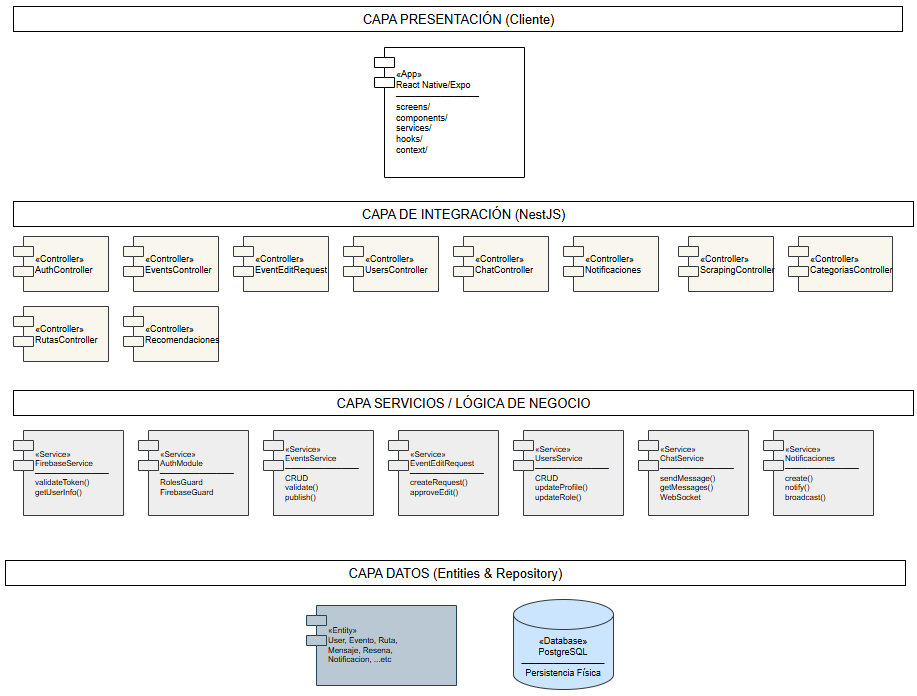
\includegraphics[width=\textwidth]{figures/vistas/vista_logica.png}
    \caption{Vista lógica del sistema Sevillaneando}
    \label{fig:vista_logica}
\end{figure}

\begin{figure}[H]
    \centering
    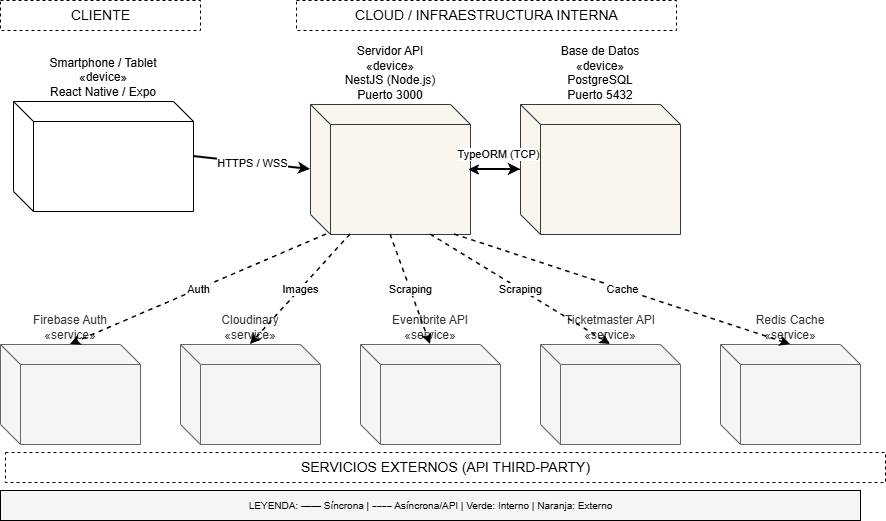
\includegraphics[width=\textwidth]{figures/vistas/vista_de_despligue.png}
    \caption{Vista de despliegue del sistema Sevillaneando}
    \label{fig:vista_despliegue}
\end{figure}

La figura~\ref{fig:conexion_tecnologias} resume cómo se conectan todas las tecnologías del sistema en tiempo de ejecución, mostrando el camino que recorre una petición desde que el usuario interactúa con la aplicación hasta que los datos son persistidos o devueltos.

\begin{figure}[H]
\centering
\begin{tikzpicture}[
    node distance=1.2cm and 2.0cm,
    every node/.style={font=\small},
    box/.style={draw, rounded corners=3pt, minimum width=2.6cm, minimum height=0.75cm, align=center, fill=white},
    ext/.style={draw, rounded corners=3pt, minimum width=2.6cm, minimum height=0.75cm, align=center, fill=gray!12},
    arr/.style={-{Stealth[length=5pt]}, thick},
    darr/.style={<->, thick, dashed},
]

% Columna izquierda: móvil
\node[box] (screen)  {Pantalla\\(React Native)};
\node[box, below=of screen] (ctx)    {Contextos\\(Auth/Socket/Tema)};
\node[box, below=of ctx]    (axios)  {Servicios\\(Axios)};
\node[box, below=of axios]  (fbase)  {Firebase SDK\\(cliente)};

% Columna central: backend
\node[box, right=3.2cm of screen]  (guard)  {FirebaseAuthGuard};
\node[box, below=of guard]         (ctrl)   {Controller\\(NestJS)};
\node[box, below=of ctrl]          (svc)    {Service\\(NestJS)};
\node[box, below=of svc]           (orm)    {TypeORM};
\node[box, below=of orm]           (db)     {PostgreSQL\\+ PostGIS};

% Columna derecha: servicios externos
\node[ext, right=2.8cm of guard]   (fbauth) {Firebase\\Authentication};
\node[ext, below=of fbauth]        (cloud)  {Cloudinary};
\node[ext, below=of cloud]         (osm)    {OpenStreetMap};
\node[ext, below=of osm]           (scrap)  {Ticketmaster\\Portal Sevilla};

% Flechas móvil → backend
\draw[arr] (axios)  -- node[above, font=\tiny] {HTTP/REST} (ctrl);
\draw[arr] (ctx)    -- node[above, font=\tiny] {WS token} (guard);

% Flechas internas backend
\draw[arr] (guard) -- (ctrl);
\draw[arr] (ctrl)  -- (svc);
\draw[arr] (svc)   -- (orm);
\draw[arr] (orm)   -- (db);

% Firebase: cliente ↔ Firebase Auth
\draw[darr] (fbase) -- node[right, font=\tiny] {JWT} (fbauth);
% Guard verifica token con Firebase
\draw[arr] (guard)  -- node[above, font=\tiny] {verifica token} (fbauth);

% Service → Cloudinary
\draw[arr] (svc)    -- node[above, font=\tiny] {upload} (cloud);

% Pantalla → OSM (tiles directos)
\draw[arr] (screen) -- node[above, font=\tiny] {tiles} (osm);

% Scheduler → scrapers (flecha punteada desde Service)
\draw[arr, dashed] (svc) -- node[above, font=\tiny] {cron} (scrap);

% Etiqueta Socket.IO
\node[font=\tiny\itshape, above=0.15cm of guard] {Socket.IO / REST};

\end{tikzpicture}
\caption{Conexión entre tecnologías del sistema en tiempo de ejecución}
\label{fig:conexion_tecnologias}
\end{figure}

\subsection{Aplicación móvil (frontend)}

La aplicación móvil actúa como único punto de interacción con el usuario. Ha sido desarrollada con \textbf{React Native} y \textbf{Expo}, lo que permite generar una única base de código compatible con Android e iOS. La arquitectura interna del frontend se estructura en cuatro niveles:

\begin{itemize}
    \item \textbf{Pantallas}: componentes que representan vistas completas navegables.
    \item \textbf{Componentes}: elementos reutilizables que componen la interfaz.
    \item \textbf{Servicios}: capa de comunicación con el backend mediante \textbf{Axios}. Todos los servicios comparten un cliente Axios centralizado que inyecta automáticamente el token de Firebase en la cabecera \texttt{Authorization} de cada petición, gestiona un \textit{timeout} global de 60 segundos y aplica un interceptor de reintento ante errores de red.
    \item \textbf{Contextos}: gestión del estado global compartido entre pantallas (\texttt{AuthContext} para la sesión, \texttt{SocketContext} para la conexión WebSocket, \texttt{ThemeContext} para el tema visual y \texttt{NotificacionesContext} para los avisos pendientes).
\end{itemize}

La navegación entre pantallas se implementa con \textbf{React Navigation} mediante una navegación en pila (\textit{stack navigator}), separando las rutas autenticadas de las públicas. El \texttt{AuthContext} determina en tiempo de montaje qué pila de navegación se activa según el estado de la sesión.

La figura~\ref{fig:flujo_frontend} muestra cómo interactúan estos niveles desde la acción del usuario hasta la respuesta del servidor.

\begin{figure}[H]
\centering
\begin{tikzpicture}[
    node distance=0.9cm and 1.8cm,
    every node/.style={font=\small},
    box/.style={draw, rounded corners=3pt, minimum width=3.0cm, minimum height=0.7cm, align=center, fill=white},
    arr/.style={-{Stealth[length=5pt]}, thick},
]
\node[box] (user)    {Usuario};
\node[box, below=of user]  (screen) {Pantalla (Screen)};
\node[box, below=of screen](svc)    {Servicio (Axios)};
\node[box, below=of svc]   (ctx)    {AuthContext\\(token Firebase)};
\node[box, below=of ctx]   (api)    {Backend API REST};
\node[box, below=of api]   (resp)   {Respuesta JSON};

\draw[arr] (user)   -- node[right, font=\tiny] {acción} (screen);
\draw[arr] (screen) -- node[right, font=\tiny] {llama} (svc);
\draw[arr] (ctx)    -- node[right, font=\tiny] {inyecta token} (svc);
\draw[arr] (svc)    -- node[right, font=\tiny] {HTTP + Bearer token} (api);
\draw[arr] (api)    -- node[right, font=\tiny] {JSON} (resp);
\draw[arr] (resp)   -- ++(3.2,0) |- node[right, font=\tiny, pos=0.25] {actualiza estado} (screen);
\end{tikzpicture}
\caption{Flujo de una petición en el frontend desde la acción del usuario hasta la actualización de la pantalla}
\label{fig:flujo_frontend}
\end{figure}

\subsection{Servidor backend}

El backend es una API REST desarrollada con \textbf{NestJS} sobre \textbf{Node.js}. NestJS organiza el servidor en módulos independientes, cada uno con sus controladores, servicios y entidades. Esta separación facilita el mantenimiento y permite extender el sistema sin afectar al resto de componentes.

Cada petición HTTP entrante pasa por la siguiente cadena de responsabilidades:

\begin{enumerate}
    \item \textbf{Guards}: \texttt{FirebaseAuthGuard} intercepta la petición, extrae el token \texttt{Bearer} de la cabecera \texttt{Authorization} y lo verifica con el SDK de administración de Firebase. Si el token es inválido o ha expirado, la petición es rechazada con \texttt{401 Unauthorized} antes de llegar al controlador.
    \item \textbf{Controlador}: recibe la petición validada, extrae los parámetros de ruta, \textit{query} y cuerpo, y delega la lógica de negocio en el servicio correspondiente.
    \item \textbf{Servicio}: ejecuta la lógica de negocio, interactúa con TypeORM para consultar o modificar la base de datos, y si es necesario llama a servicios externos (Cloudinary para imágenes, Firebase Admin para notificaciones).
    \item \textbf{TypeORM}: traduce las operaciones del servicio en consultas SQL optimizadas y gestiona la conexión con PostgreSQL.
\end{enumerate}

La figura~\ref{fig:flujo_backend} ilustra esta cadena para una petición autenticada típica.

\begin{figure}[H]
\centering
\begin{tikzpicture}[
    node distance=0.5cm and 2.2cm,
    every node/.style={font=\small},
    box/.style={draw, rounded corners=3pt, minimum width=3.2cm, minimum height=0.7cm, align=center, fill=white},
    ext/.style={draw, rounded corners=3pt, minimum width=2.8cm, minimum height=0.7cm, align=center, fill=gray!12},
    arr/.style={-{Stealth[length=5pt]}, thick},
]
\node[box] (req)   {Petición HTTP};
\node[box, below=of req]   (guard)  {FirebaseAuthGuard};
\node[box, below=of guard] (ctrl)   {Controller};
\node[box, below=of ctrl]  (svc)    {Service};
\node[box, below=of svc]   (orm)    {TypeORM};
\node[box, below=of orm]   (db)     {PostgreSQL + PostGIS};

\node[ext, right=2.6cm of guard] (fbadmin) {Firebase Admin SDK};
\node[ext, right=2.6cm of svc]   (cld)     {Cloudinary};

\draw[arr] (req)   -- (guard);
\draw[arr] (guard) -- node[right, font=\tiny] {token OK} (ctrl);
\draw[arr] (ctrl)  -- (svc);
\draw[arr] (svc)   -- (orm);
\draw[arr] (orm)   -- (db);

\draw[arr] (guard) -- node[above, font=\tiny] {verifica} (fbadmin);
\draw[arr] (svc)   -- node[above, font=\tiny] {upload/delete} (cld);
\end{tikzpicture}
\caption{Cadena de responsabilidades en el backend para una petición autenticada}
\label{fig:flujo_backend}
\end{figure}

Además de la API REST, el backend integra un servidor \textbf{Socket.IO} para la comunicación en tiempo real del chat. La conexión WebSocket se autentica en el \textit{handshake} inicial mediante el mismo mecanismo que la API REST: el cliente envía el token de Firebase como parámetro de la URL de conexión, y el middleware de Socket.IO lo verifica antes de aceptar la conexión. Una vez autenticada, la conexión se mantiene abierta y el servidor puede emitir eventos al cliente en cualquier momento sin necesidad de una nueva petición.

\subsection{Base de datos}

La persistencia de datos se gestiona con \textbf{PostgreSQL 15} junto con la extensión \textbf{PostGIS}. PostgreSQL cubre el modelo relacional general del sistema, mientras que PostGIS añade soporte para datos geográficos, permitiendo almacenar coordenadas como puntos \texttt{geography} en SRID 4326 y ejecutar consultas espaciales eficientes como el filtrado por radio (\texttt{ST\_DWithin}) o el cálculo de distancias en metros (\texttt{ST\_Distance}). La comunicación entre el backend y la base de datos se realiza a través de \textbf{TypeORM}, que mapea las entidades TypeScript a tablas SQL y genera las consultas correspondientes.

\subsection{Servicios externos}

El sistema delega en servicios externos las siguientes responsabilidades:

\begin{itemize}
    \item \textbf{Firebase Authentication}: gestión del ciclo de vida de la sesión del usuario (registro, inicio de sesión y tokens JWT). El cliente móvil usa el SDK de Firebase para obtener y renovar tokens; el backend usa el SDK de administración para verificarlos sin almacenar contraseñas ni gestionar sesiones propias.
    \item \textbf{Cloudinary}: almacenamiento y servicio de imágenes asociadas a eventos, perfiles y chats. El backend sube las imágenes directamente a Cloudinary mediante su SDK y almacena únicamente la URL resultante en PostgreSQL. Cloudinary sirve las imágenes desde su CDN con transformaciones automáticas de formato y calidad.
    \item \textbf{OpenStreetMap}: visualización de mapas interactivos en el frontend mediante \texttt{react-native-maps}. Los \textit{tiles} cartográficos se obtienen directamente del servidor de OpenStreetMap sin pasar por el backend.
    \item \textbf{Ticketmaster / Portal municipal de Sevilla}: fuentes externas de eventos consultadas automáticamente mediante scraping. El backend ejecuta diariamente un \textit{cron job} que invoca cada scraper, transforma los datos al modelo interno y los persiste en PostgreSQL asignándolos al usuario técnico \textit{scraper-bot}.
\end{itemize}

La figura~\ref{fig:flujo_autenticacion} muestra en detalle el flujo completo de autenticación, desde el inicio de sesión del usuario hasta la verificación del token en el backend.

\begin{figure}[H]
\centering
\begin{tikzpicture}[
    node distance=1.0cm and 2.4cm,
    every node/.style={font=\small},
    box/.style={draw, rounded corners=3pt, minimum width=3.0cm, minimum height=0.72cm, align=center, fill=white},
    ext/.style={draw, rounded corners=3pt, minimum width=3.0cm, minimum height=0.72cm, align=center, fill=gray!12},
    arr/.style={-{Stealth[length=5pt]}, thick},
]
% Columna izquierda
\node[box] (app)    {App móvil};
\node[box, below=of app]  (sdk)    {Firebase SDK (cliente)};
\node[box, below=2.5cm of sdk]  (axios)  {Axios (interceptor)};
\node[box, below=of axios] (be)     {Backend NestJS};
\node[box, below=of be]    (guard)  {FirebaseAuthGuard};

% Columna derecha
\node[ext, right=3.0cm of sdk]   (fbauth) {Firebase Authentication};
\node[ext, right=3.0cm of guard] (fbadm)  {Firebase Admin SDK};

% Flechas
\draw[arr] (app)   -- node[right, font=\tiny] {email + pass} (sdk);
\draw[arr] (sdk)   -- node[above, font=\tiny] {signIn()} (fbauth);
\draw[arr] (fbauth) -- node[above, font=\tiny] {JWT (60 min)} (sdk);
\draw[arr] (sdk)   -- node[right, font=\tiny] {token} (axios);
\draw[arr] (axios) -- node[right, font=\tiny] {Authorization: Bearer \{token\}} (be);
\draw[arr] (be)    -- (guard);
\draw[arr] (guard) -- node[above, font=\tiny] {verifyIdToken()} (fbadm);
\draw[arr] (fbadm) -- node[above, font=\tiny] {uid + claims} (guard);
\end{tikzpicture}
\caption{Flujo de autenticación: desde el inicio de sesión hasta la verificación del token en el backend}
\label{fig:flujo_autenticacion}
\end{figure}

\section{Modelo de datos}

El modelo de datos del sistema refleja las entidades identificadas en el análisis y las relaciones entre ellas. A continuación se describen las entidades principales y sus atributos más relevantes.

\subsection{Usuario (\texttt{User})}

Representa a cada persona registrada en el sistema. Sus atributos principales son el identificador UUID, el UID de Firebase, el correo electrónico, el nombre, la foto de perfil, la ubicación geográfica (punto PostGIS en SRID 4326), el rol (\texttt{user}, \texttt{moderator} o \texttt{admin}) y el array de intereses por categoría (\texttt{intereses}). Adicionalmente, almacena preferencias de personalización como el orden de categorías (\texttt{categoryOrder}) y los radios de búsqueda configurados (\texttt{radiusOptions}).

\subsection{Evento (\texttt{Event})}

Representa un evento cultural o de ocio. Sus atributos incluyen título, descripción, dirección, ubicación geográfica (punto PostGIS en SRID 4326), fechas de inicio y fin, precio (fijo o en rango), imágenes, estado de moderación (\texttt{Pendiente}, \texttt{Aprobado} o \texttt{Rechazado}), visibilidad (\texttt{privado}), enlace de acceso (\texttt{linkAcceso}) para eventos privados y recurrencia (\texttt{diario}, \texttt{semanal}, \texttt{quincenal} o \texttt{mensual}).

\subsection{Categoría (\texttt{Categoria})}

Clasifica los eventos por temática. Contiene nombre y descripción y es gestionada exclusivamente por los administradores.

\subsection{Reseña (\texttt{Resena})}

Permite a los usuarios valorar eventos. Incluye puntuación de 1 a 5 estrellas y comentario opcional, referenciando al usuario autor y al evento valorado.

\subsection{Mensaje de evento (\texttt{Mensaje})}

Almacena los mensajes del chat grupal asociado a cada evento. Incluye el contenido de texto, una URL de imagen opcional, el usuario emisor y la referencia al evento.

\subsection{Mensaje privado (\texttt{MensajePrivado})}

Representa las conversaciones directas entre dos usuarios. Contiene el contenido, imagen opcional, referencias a emisor y receptor, y un indicador de lectura (\texttt{leido}).

\subsection{Notificación (\texttt{Notificacion})}

Registra los avisos enviados a cada usuario. Incluye el tipo de notificación (aprobación, rechazo, evento cercano, evento próximo, mensaje privado, nuevo seguidor o recomendación), el mensaje y el estado de lectura.

\subsection{Ruta (\texttt{Ruta})}

Agrupa una secuencia ordenada de eventos formando un itinerario. Almacena el título, la descripción, la secuencia de eventos, el trayecto geográfico (array de puntos), la temporización estimada en minutos, el creador y la puntuación promedio obtenida de las valoraciones de otros usuarios.

\subsection{Recomendación (\texttt{Recomendacion})}

Almacena las sugerencias personalizadas generadas por el motor de recomendaciones para cada usuario, incluyendo los eventos recomendados, los criterios aplicados y si ya han sido visualizadas.

\subsection{Solicitud de edición (\texttt{EventEditRequest})}

Permite a los moderadores proponer cambios sobre un evento sin aplicarlos directamente. Incluye los campos modificados, el estado de la solicitud (\texttt{pendiente}, \texttt{aprobada} o \texttt{rechazada}) y, en caso de rechazo, el motivo.

\subsection{Diagrama entidad-relación}

La figura~\ref{fig:edt_modelo} muestra el diagrama entidad-relación del sistema con las relaciones principales entre entidades.

\begin{figure}[H]
    \centering
    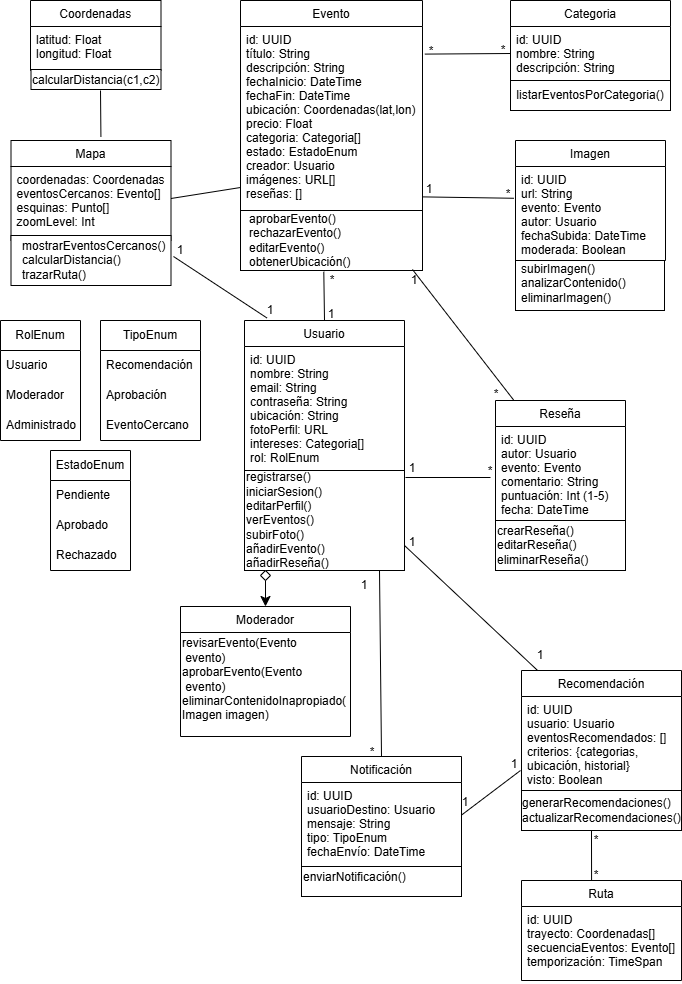
\includegraphics[width=0.95\textwidth]{figures/vistas/vista_de_datos.png}
    \caption{Diagrama entidad-relación del sistema}
    \label{fig:edt_modelo}
\end{figure}

Las relaciones principales entre entidades son las siguientes:

\begin{itemize}
    \item Un usuario puede crear múltiples eventos (1:N).
    \item Un usuario puede asistir, guardar, compartir o visitar múltiples eventos (M:N).
    \item Un evento pertenece a una categoría (N:1).
    \item Un evento puede tener múltiples reseñas y mensajes (1:N).
    \item Un usuario puede seguir a otros usuarios (M:N reflexiva).
    \item Una ruta contiene una secuencia de eventos (M:N).
    \item Una recomendación agrupa múltiples eventos para un usuario concreto (M:N).
\end{itemize}

\section{Diseño de la API REST}

El backend expone una API REST cuya organización sigue la estructura modular de NestJS. Cada módulo define un conjunto de endpoints agrupados por recurso. La tabla~\ref{tab:api} muestra los módulos principales y sus operaciones más relevantes.

\begin{table}[H]
\centering
\caption{Módulos y operaciones principales de la API REST}
\label{tab:api}
\resizebox{\textwidth}{!}{%
\begin{tabular}{|l|l|l|}
\hline
\textbf{Módulo} & \textbf{Método / Ruta} & \textbf{Descripción} \\
\hline
\multirow{8}{*}{Eventos} & POST /events & Crear evento \\
 & GET /events & Listar eventos (con filtros) \\
 & GET /events/:id & Detalle de evento \\
 & PUT /events/:id & Editar evento \\
 & DELETE /events/:id & Eliminar evento \\
 & PATCH /events/:id/aprobar & Aprobar evento (moderador/admin) \\
 & GET /events/acceso/:linkAcceso & Acceder a evento privado por enlace \\
 & GET /events/:id/private-share-link & Generar enlace de acceso privado \\
\hline
\multirow{4}{*}{Usuarios} & GET /users/me & Perfil del usuario autenticado \\
 & GET /users/search & Buscar usuarios \\
 & PATCH /users/:id & Actualizar perfil \\
 & PATCH /users/:id/role & Cambiar rol (admin) \\
\hline
\multirow{2}{*}{Categorías} & GET /categorias & Listar categorías \\
 & POST /categorias & Crear categoría (admin) \\
\hline
\multirow{2}{*}{Rutas} & GET /rutas & Listar rutas \\
 & POST /rutas & Crear ruta \\
\hline
Recomendaciones & GET /recomendaciones & Obtener recomendaciones personalizadas \\
\hline
Notificaciones & GET /notificaciones & Listar notificaciones del usuario \\
\hline
\end{tabular}%
}
\end{table}

Todos los endpoints que requieren autenticación reciben el token de Firebase en la cabecera \texttt{Authorization: Bearer <token>}. Los endpoints que exigen rol de moderador o administrador aplican un guard adicional de roles.

La API aplica limitación de velocidad (\textit{throttling}) mediante \texttt{@nestjs/throttler} con tres niveles configurables:

\begin{itemize}
    \item \textbf{Estricto} (5 req/min): operaciones sensibles como registro de cuenta.
    \item \textbf{Moderado} (20 req/min): escrituras habituales.
    \item \textbf{Subida} (10 req/min): carga de imágenes.
\end{itemize}

\section{Diseño del sistema de moderación}

La moderación de eventos públicos es una de las piezas centrales del sistema. La figura~\ref{fig:secuencias_moderacion} muestra el diagrama de secuencias del flujo de moderación de un evento público.

\begin{figure}[H]
    \centering
    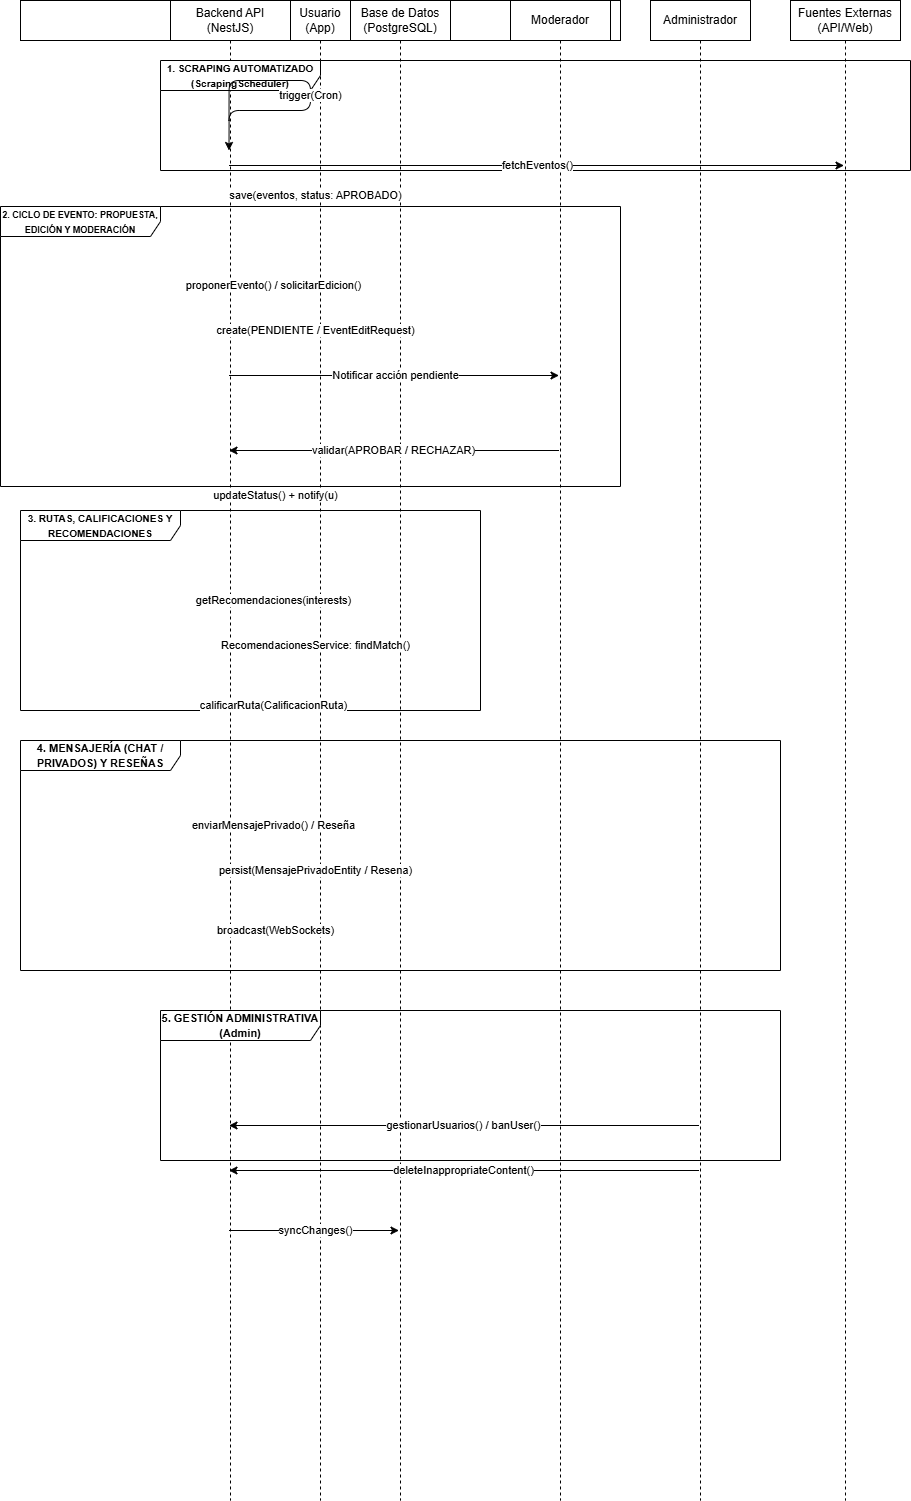
\includegraphics[width=\textwidth]{figures/vistas/vista_de_secuencias.png}
    \caption{Diagrama de secuencias del flujo de moderación de un evento}
    \label{fig:secuencias_moderacion}
\end{figure}

El flujo de estados de un evento sigue las siguientes reglas de negocio:

\begin{itemize}
    \item Al crear un evento público, su estado inicial es \textbf{Pendiente}.
    \item Un evento privado se aprueba automáticamente y es accesible solo mediante enlace.
    \item Un moderador puede aprobar (\textbf{Aprobado}) o rechazar (\textbf{Rechazado}) un evento pendiente.
    \item Al editar un evento público ya aprobado, este vuelve a estado \textbf{Pendiente} y desaparece del listado público hasta ser revisado de nuevo.
    \item Si un evento privado se cambia a público, pasa a \textbf{Pendiente} y entra en el flujo de moderación.
    \item Si un evento público se cambia a privado, se aprueba automáticamente y se genera un enlace de acceso.
    \item Los eventos privados que se editan sin cambiar de visibilidad se actualizan directamente sin pasar por moderación.
\end{itemize}

El listado general de eventos solo muestra eventos públicos aprobados y eventos privados únicamente al creador o a quien disponga del enlace. El listado de edición del usuario muestra sus eventos creados que no están en moderación. El listado de moderación muestra los eventos públicos pendientes.

Adicionalmente, los moderadores pueden crear solicitudes de edición (\texttt{EventEditRequest}) proponiendo cambios al creador del evento. El creador recibe una notificación y puede aceptar o rechazar la propuesta. Al aprobar o rechazar un evento, el moderador desaparece del listado de moderación.

En cuanto al comportamiento del botón de compartir, en eventos públicos cualquier usuario puede compartirlo. En eventos privados, el botón de compartir se sustituye por uno de \textit{invitar}, que solo está activo para el creador del evento; el resto de usuarios lo ven desactivado.

\section{Diseño de la interfaz de usuario}

\subsection{Principios de diseño}

La interfaz de usuario ha sido diseñada siguiendo los principios de usabilidad para aplicaciones móviles:

\begin{itemize}
    \item \textbf{Consistencia visual}: se utiliza un sistema de componentes temáticos (\texttt{ThemedView}, \texttt{ThemedCard}, \texttt{ThemedButton}, \texttt{ThemedText}) que garantizan una apariencia coherente en todas las pantallas, tanto en modo claro como en modo oscuro.
    \item \textbf{Adaptabilidad}: la aplicación soporta modo claro y modo oscuro, adaptándose automáticamente a la preferencia del sistema o permitiendo el cambio manual desde el perfil.
    \item \textbf{Jerarquía de información}: cada pantalla prioriza la información más relevante para el usuario, ocultando las opciones avanzadas o de administración según el rol.
    \item \textbf{Accesibilidad de acciones}: las acciones principales (apuntarse, guardar, compartir) están siempre visibles en el detalle de evento sin necesidad de desplazarse.
\end{itemize}

\subsection{Grafo de navegación}

La aplicación se divide en dos grupos de pantallas según el estado de autenticación del usuario. La figura~\ref{fig:grafo_navegacion} muestra el grafo de navegación completo.

\begin{figure}[H]
    \centering
    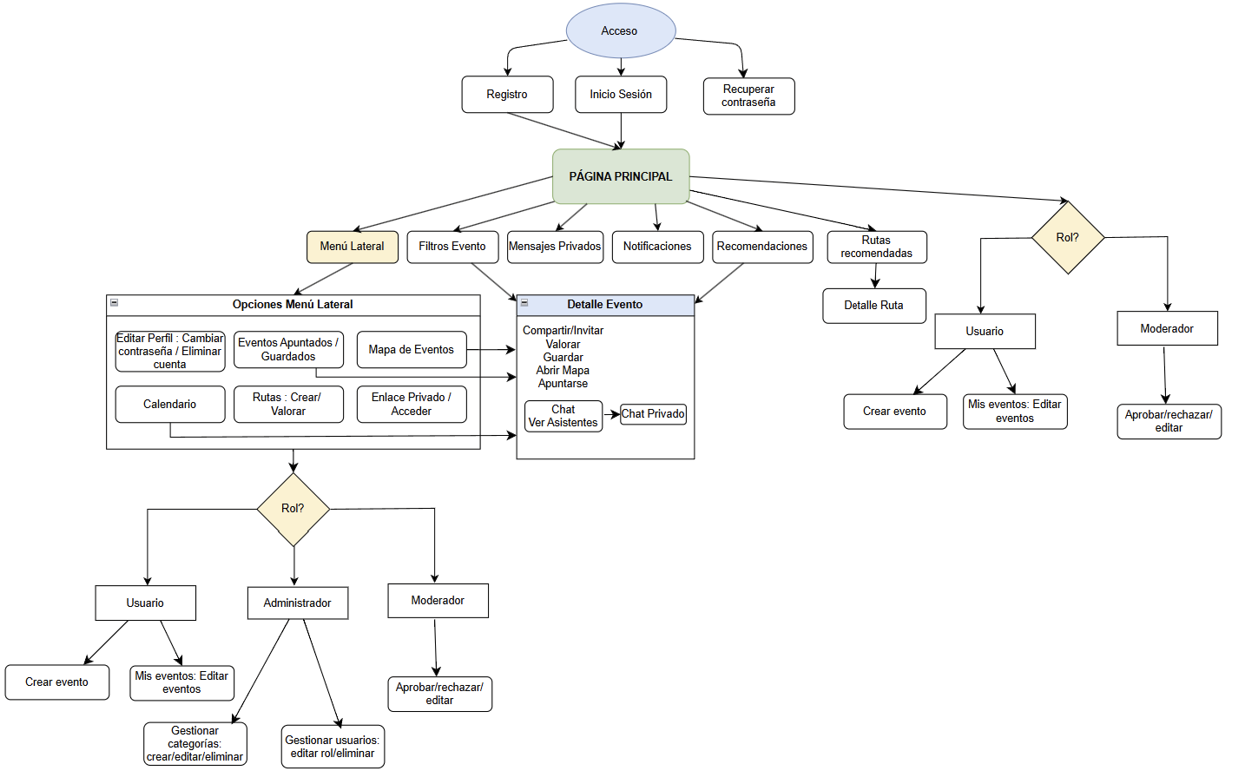
\includegraphics[width=\textwidth]{figures/grafo_navegacion.png}
    \caption{Grafo de navegación de la aplicación}
    \label{fig:grafo_navegacion}
\end{figure}

El grupo de pantallas no autenticadas comprende únicamente las pantallas de inicio de sesión y registro. El grupo de pantallas autenticadas incluye todas las funcionalidades de la aplicación, organizadas alrededor de la pantalla principal.

Las pantallas exclusivas de moderador y administrador solo son accesibles si el usuario dispone del rol correspondiente; de lo contrario, no aparecen en el menú lateral ni en ningún punto de entrada de la navegación.

\subsection{Pantallas principales}

La tabla~\ref{tab:pantallas} describe las pantallas del sistema y su accesibilidad según el rol del usuario.

\begin{table}[H]
\centering
\caption{Pantallas del sistema y roles que pueden acceder}
\label{tab:pantallas}
\resizebox{\textwidth}{!}{%
\begin{tabular}{|l|l|c|}
\hline
\textbf{Pantalla} & \textbf{Descripción} & \textbf{Rol mínimo} \\
\hline
Inicio de sesión & Autenticación con correo y contraseña & No autenticado \\
Registro & Creación de cuenta nueva & No autenticado \\
Pantalla principal & Listado de eventos con filtros y recomendaciones & Todos \\
Detalle de evento & Información completa, chat, reseñas y asistencia & Todos \\
Mapa de eventos & Vista cartográfica de los eventos cercanos & Todos \\
Calendario & Eventos con fecha a los que está apuntado el usuario & Todos \\
Acceso a evento privado & Acceso a evento privado mediante enlace de invitación & Todos \\
Crear evento & Formulario de creación de evento público o privado & Usuario \\
Editar evento & Modificación de un evento propio & Usuario \\
Mis eventos & Listado de eventos creados por el usuario & Usuario \\
Guardados y privados & Eventos guardados y eventos privados del usuario & Usuario \\
Rutas & Listado de rutas públicas & Todos \\
Detalle de ruta & Información de la ruta y secuencia de eventos & Todos \\
Rutas recomendadas & Itinerarios generados automáticamente para el usuario & Usuario \\
Crear ruta & Formulario para crear una ruta propia & Usuario \\
Notificaciones & Listado de notificaciones del usuario & Usuario \\
Mensajes & Lista de conversaciones privadas & Usuario \\
Mensaje directo & Chat privado entre dos usuarios & Usuario \\
Perfil de usuario & Vista del perfil de otro usuario & Usuario \\
Amigos & Seguidores y seguidos del usuario & Usuario \\
Editar perfil & Modificación de datos personales e intereses & Usuario \\
Cambiar contraseña & Modificación de la contraseña de la cuenta & Usuario \\
Panel de administración & Gestión de usuarios y roles & Administrador \\
Gestión de categorías & Creación, edición y eliminación de categorías & Administrador \\
Moderación de eventos & Revisión y aprobación de eventos pendientes & Moderador \\
Edición moderada & Propuesta de cambios sobre un evento pendiente & Moderador \\
\hline
\end{tabular}%
}
\end{table}

\subsection{Capturas de pantalla}

Las siguientes figuras muestran las pantallas más representativas de la aplicación.

\begin{figure}[H]
    \centering
    \begin{minipage}[b]{0.32\textwidth}
        \centering
        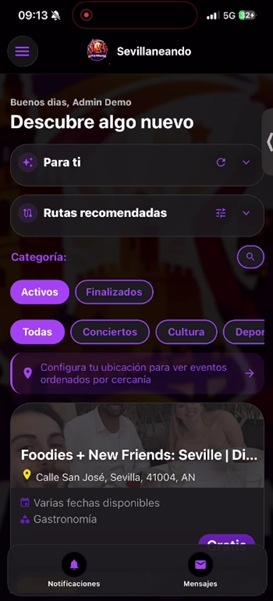
\includegraphics[width=\textwidth]{figures/home_screen.png}
        \caption{Pantalla principal}
        \label{fig:home}
    \end{minipage}
    \hfill
    \begin{minipage}[b]{0.32\textwidth}
        \centering
        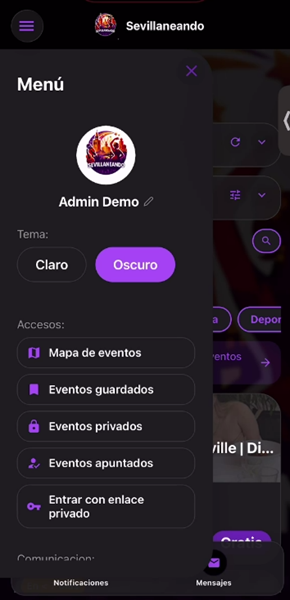
\includegraphics[width=\textwidth]{figures/lateral_menu.png}
        \caption{Menú lateral}
        \label{fig:lateral_menu}
    \end{minipage}
    \hfill
    \begin{minipage}[b]{0.32\textwidth}
        \centering
        
\includegraphics[width=\textwidth]{figures/paso5/event_detail.png}
        \caption{Detalle de evento}
        \label{fig:event_detail}
    \end{minipage}
\end{figure}

\begin{figure}[H]
    \centering
    \begin{minipage}[b]{0.32\textwidth}
        \centering
        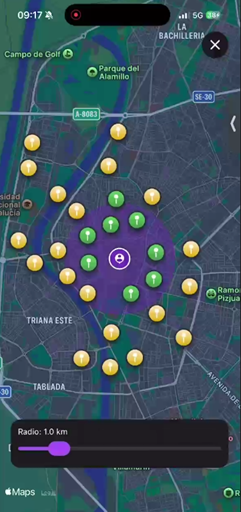
\includegraphics[width=\textwidth]{figures/paso3/mapa1.png}
        \caption{Mapa de eventos}
        \label{fig:mapa}
    \end{minipage}
    \hfill
    \begin{minipage}[b]{0.32\textwidth}
        \centering
        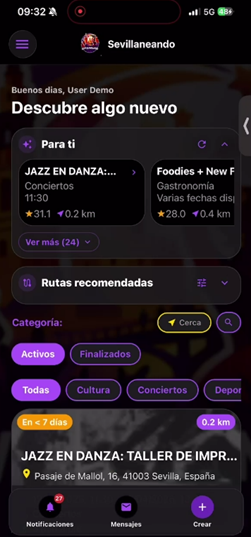
\includegraphics[width=\textwidth]{figures/paso8/recomendados.png}
        \caption{Eventos recomendados}
        \label{fig:recomendados}
    \end{minipage}
    \hfill
    \begin{minipage}[b]{0.32\textwidth}
        \centering
        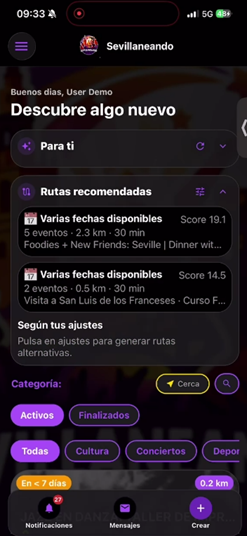
\includegraphics[width=\textwidth]{figures/paso8/rutas_recomendadas.png}
        \caption{Rutas recomendadas}
        \label{fig:rutas_rec}
    \end{minipage}
\end{figure}

\begin{figure}[H]
    \centering
    \begin{minipage}[b]{0.32\textwidth}
        \centering
        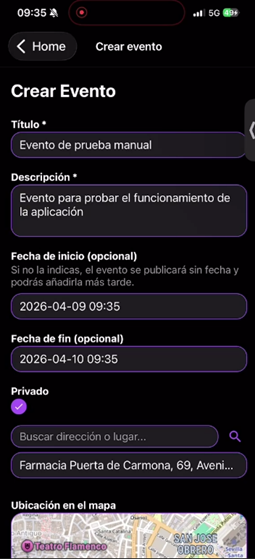
\includegraphics[width=\textwidth]{figures/paso10/crear_evento.png}
        \caption{Formulario de creación de evento}
        \label{fig:crear_evento}
    \end{minipage}
    \hfill
    \begin{minipage}[b]{0.32\textwidth}
        \centering
        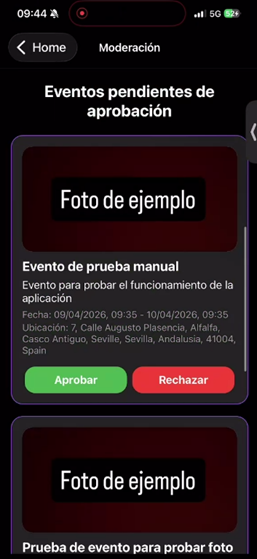
\includegraphics[width=\textwidth]{figures/paso14/moderacion.png}
        \caption{Panel de moderación}
        \label{fig:moderacion}
    \end{minipage}
    \hfill
    \begin{minipage}[b]{0.32\textwidth}
        \centering
        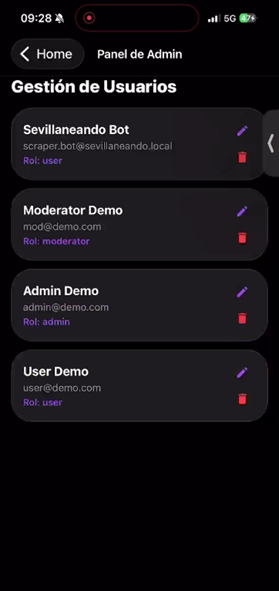
\includegraphics[width=\textwidth]{figures/paso7/panel_admin.png}
        \caption{Panel de administración}
        \label{fig:admin}
    \end{minipage}
\end{figure}

\begin{figure}[H]
    \centering
    \begin{minipage}[b]{0.32\textwidth}
        \centering
        
\includegraphics[width=\textwidth]{figures/paso16/chat_evento.png}
        \caption{Chat de evento}
        \label{fig:chat_evento}
    \end{minipage}
    \hfill
    \begin{minipage}[b]{0.32\textwidth}
        \centering
        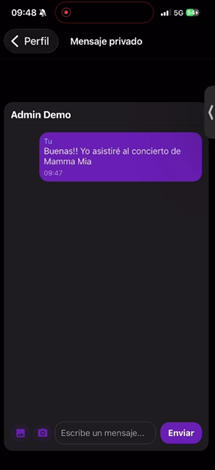
\includegraphics[width=\textwidth]{figures/paso16/chat_priv.png}
        \caption{Mensaje directo}
        \label{fig:chat_priv}
    \end{minipage}
    \hfill
    \begin{minipage}[b]{0.32\textwidth}
        \centering
        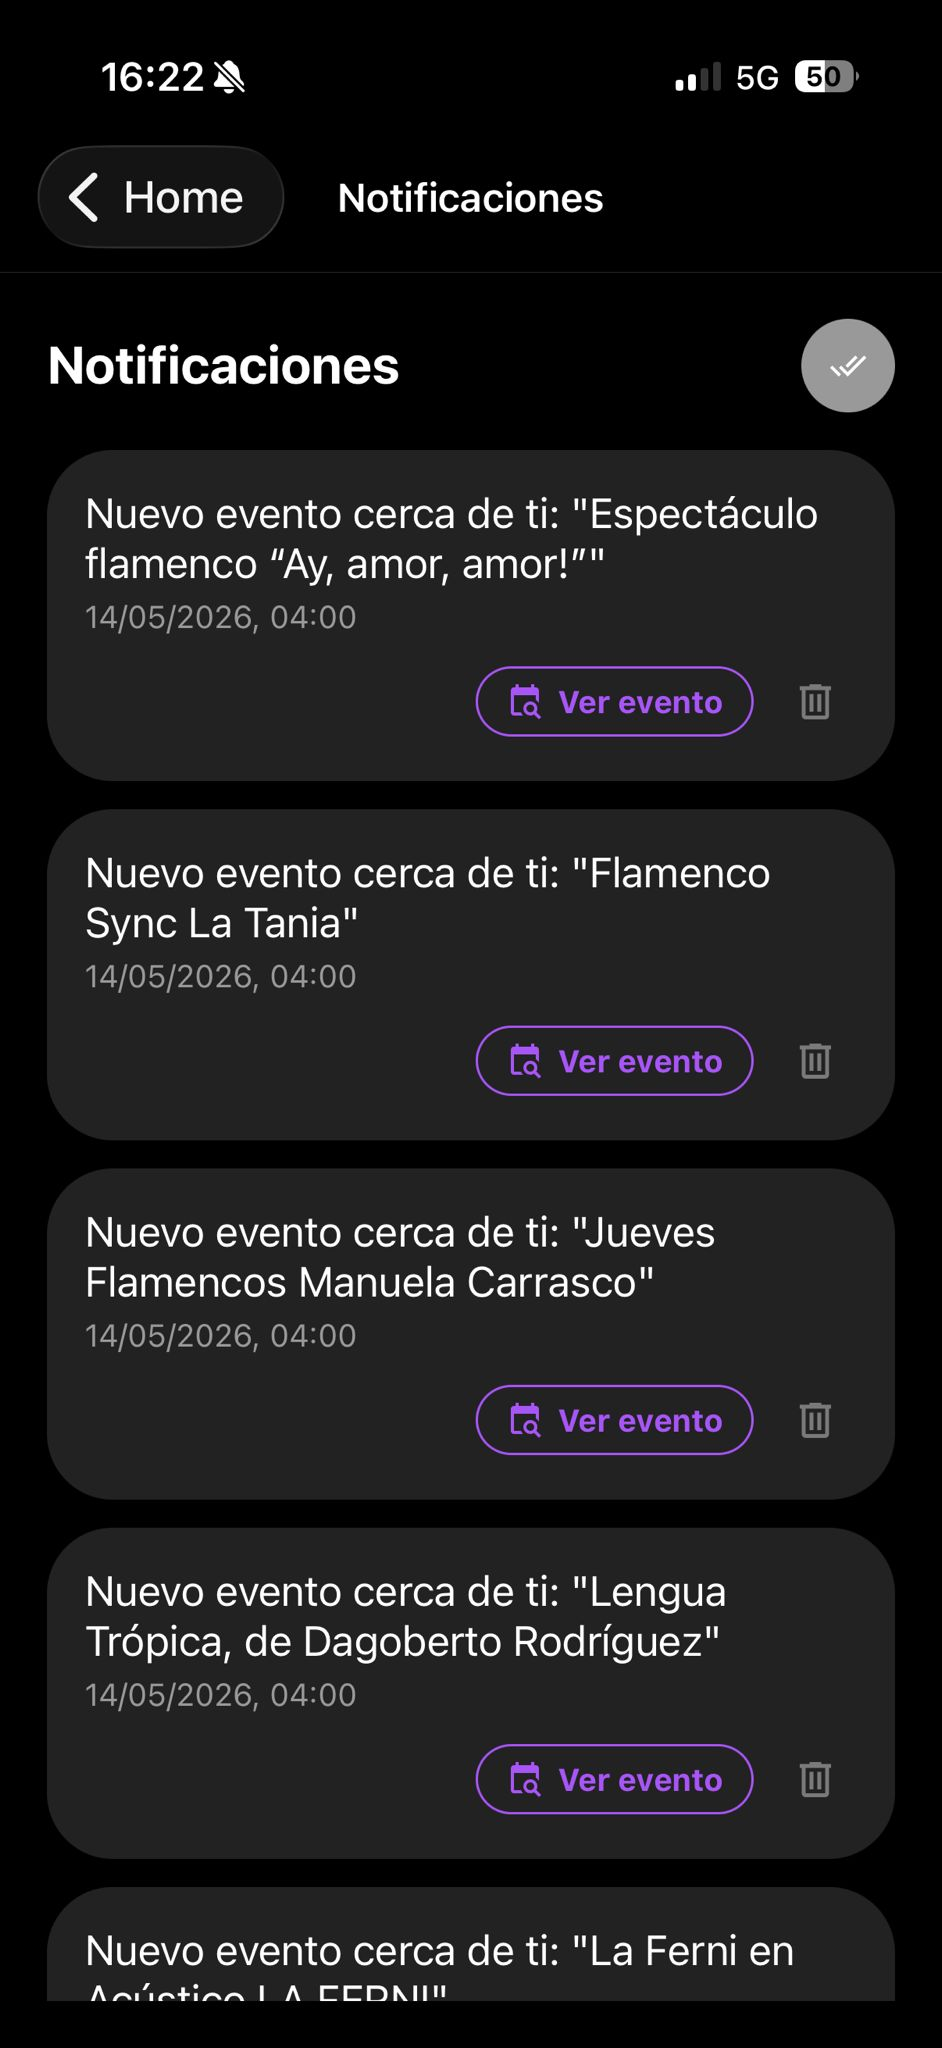
\includegraphics[width=\textwidth]{figures/paso15/notificaciones.png}
        \caption{Notificaciones}
        \label{fig:notificaciones}
    \end{minipage}
\end{figure}

\begin{figure}[H]
    \centering
    \begin{minipage}[b]{0.32\textwidth}
        \centering
        
\includegraphics[width=\textwidth]{figures/paso11/evento_privado.png}
        \caption{Evento privado en listado}
        \label{fig:evento_priv_listado}
    \end{minipage}
    \hfill
    \begin{minipage}[b]{0.32\textwidth}
        \centering
        
\includegraphics[width=\textwidth]{figures/paso11/detalles_event_priv.png}
        \caption{Detalle de evento privado}
        \label{fig:evento_priv_detalle}
    \end{minipage}
    \hfill
    \begin{minipage}[b]{0.32\textwidth}
        \centering
        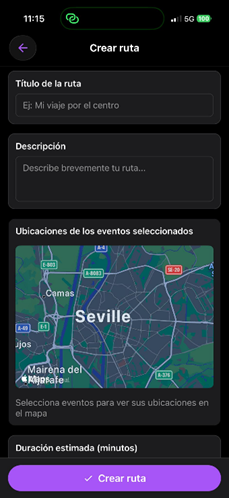
\includegraphics[width=\textwidth]{figures/paso9/crear_ruta.png}
        \caption{Creación de ruta}
        \label{fig:crear_ruta}
    \end{minipage}
\end{figure}

\section{Diseño del sistema de comunicación en tiempo real}

El chat de la aplicación está implementado sobre \textbf{Socket.IO}, integrado en el mismo servidor NestJS que la API REST. Se definen dos canales de comunicación independientes:

\begin{itemize}
    \item \textbf{Chat de evento}: sala identificada por \texttt{event:\{eventId\}} en la que todos los asistentes pueden leer y enviar mensajes.
    \item \textbf{Mensajes privados}: sala personal identificada por \texttt{user:\{userId\}} que enruta los mensajes directos entre dos usuarios.
\end{itemize}

La conexión WebSocket se autentica con el mismo token de Firebase que los endpoints REST, verificado en el middleware del socket antes de aceptar la conexión. Para prevenir el abuso, el servidor aplica un límite de 10 mensajes por ventana de 10 segundos por conexión.

La figura~\ref{fig:flujo_socket} muestra el flujo completo desde el establecimiento de la conexión hasta la recepción del mensaje en otro cliente.

\begin{figure}[H]
\centering
\begin{tikzpicture}[
    node distance=0.85cm and 2.0cm,
    every node/.style={font=\small},
    box/.style={draw, rounded corners=3pt, minimum width=3.2cm, minimum height=0.7cm, align=center, fill=white},
    ext/.style={draw, rounded corners=3pt, minimum width=3.0cm, minimum height=0.7cm, align=center, fill=gray!12},
    arr/.style={-{Stealth[length=5pt]}, thick},
    darr/.style={{Stealth[length=5pt]}-{Stealth[length=5pt]}, thick, dashed},
]
\node[box] (clientA) {Cliente A\\(app móvil)};
\node[box, below=of clientA]  (ctxA)   {SocketContext};
\node[box, below=of ctxA]     (mid)    {Middleware Socket.IO\\(verifica token Firebase)};
\node[box, below=of mid]      (gate)   {ChatGateway (NestJS)};
\node[box, below=of gate]     (svcMsg) {MensajesService};
\node[box, below=of svcMsg]   (db)     {PostgreSQL};

\node[box, right=3.2cm of gate]   (sala)   {Sala: event:\{id\}\\o user:\{id\}};
\node[box, right=3.2cm of ctxA]   (clientB){Cliente B\\(app móvil)};

\node[ext, left=2.6cm of mid]    (fbadm)  {Firebase Admin SDK};

% Flechas verticales izquierda
\draw[arr] (clientA) -- node[right, font=\tiny] {connect(token)} (ctxA);
\draw[arr] (ctxA)    -- node[right, font=\tiny] {WS handshake} (mid);
\draw[arr] (mid)     -- node[right, font=\tiny] {conexión aceptada} (gate);
\draw[arr] (gate)    -- node[right, font=\tiny] {persiste} (svcMsg);
\draw[arr] (svcMsg)  -- node[right, font=\tiny] {INSERT} (db);

% Verificación token
\draw[arr] (mid) -- node[above, font=\tiny] {verifyIdToken()} (fbadm);

% Sala y emit
\draw[arr] (gate) -- node[above, font=\tiny] {join room} (sala);
\draw[arr] (sala) -- node[above, font=\tiny] {emit evento} (clientB);
\end{tikzpicture}
\caption{Flujo de comunicación en tiempo real mediante Socket.IO: conexión, autenticación y entrega de mensajes}
\label{fig:flujo_socket}
\end{figure}

\section{Diseño del sistema de recomendaciones}

El motor de recomendaciones es un componente del backend que genera listas de eventos personalizadas para cada usuario. Su diseño se basa en un algoritmo de puntuación multifactorial: cada evento candidato recibe una puntuación calculada como suma ponderada de varios factores relacionados con el comportamiento del usuario, sus intereses declarados, la proximidad temporal y la proximidad geográfica.

Los factores con mayor peso en el diseño son la afinidad por categoría (hasta 12 puntos), el haber guardado previamente el evento (+10) y la proximidad temporal al evento (hasta 8 puntos). Los eventos se ordenan de mayor a menor puntuación y se devuelven los más relevantes.

La figura~\ref{fig:flujo_recomendaciones} muestra las entradas que consulta el motor y el proceso de puntuación hasta producir la lista final.

\begin{figure}[H]
\centering
\begin{tikzpicture}[
    node distance=0.8cm and 1.6cm,
    every node/.style={font=\small},
    box/.style={draw, rounded corners=3pt, minimum width=3.2cm, minimum height=0.7cm, align=center, fill=white},
    input/.style={draw, rounded corners=3pt, minimum width=2.8cm, minimum height=0.65cm, align=center, fill=gray!10},
    arr/.style={-{Stealth[length=5pt]}, thick},
]
% Entradas
\node[input] (u1) {Intereses del usuario\\(categorías)};
\node[input, below=of u1] (u2) {Eventos asistidos\\y guardados};
\node[input, below=of u2] (u3) {Ubicación del usuario\\(punto PostGIS)};
\node[input, below=of u3] (u4) {Fecha actual};

% Motor
\node[box, right=2.6cm of u2] (motor) {Motor de puntuación\\multifactorial};

% Salida
\node[box, right=2.4cm of motor] (rank)  {Lista ordenada\\por puntuación};
\node[box, above=of rank]        (evtos) {Eventos candidatos\\(PostgreSQL)};

\draw[arr] (u1) -- (motor);
\draw[arr] (u2) -- (motor);
\draw[arr] (u3) -- (motor);
\draw[arr] (u4) -- (motor);
\draw[arr] (evtos) -- (motor);
\draw[arr] (motor) -- (rank);
\end{tikzpicture}
\caption{Entradas y proceso del motor de recomendaciones}
\label{fig:flujo_recomendaciones}
\end{figure}

El mismo motor puede generar rutas recomendadas aplicando tres estrategias seleccionables:

\begin{itemize}
    \item \textbf{balanced}: equilibra puntuación y distancia recorrida entre eventos.
    \item \textbf{walkable}: minimiza la distancia total del itinerario.
    \item \textbf{score}: maximiza la puntuación agregada de los eventos incluidos.
\end{itemize}

\section{Decisiones de diseño relevantes}

A lo largo del proceso de diseño se tomaron una serie de decisiones que merecen una justificación explícita, ya que no son evidentes a partir de los requisitos y condicionan la arquitectura y el comportamiento de la aplicación.

\subsection{Por qué tres roles y no más ni menos}

El sistema define tres roles: \textbf{usuario}, \textbf{moderador} y \textbf{administrador}. Esta jerarquía mínima responde a la necesidad de separar tres tipos de responsabilidad claramente diferenciados:

\begin{itemize}
    \item El \textbf{usuario} es el actor principal del sistema: crea, consulta y consume contenido. No tiene autoridad sobre el contenido de otros ni sobre la configuración del sistema.
    \item El \textbf{moderador} actúa como filtro de calidad: revisa y valida eventos antes de que sean visibles públicamente. Requiere más permisos que un usuario ordinario pero no debe tener acceso a la gestión del sistema, lo que delimita claramente su responsabilidad.
    \item El \textbf{administrador} gestiona la estructura del sistema (roles y categorías) pero no interviene en el contenido concreto. Esta separación evita que una única persona acumule tanto la capacidad de gestionar usuarios como la de aprobar contenido, reduciendo el riesgo de abusos y errores.
\end{itemize}

Añadir más roles (por ejemplo, un \textit{superadmin} o un \textit{editor}) habría incrementado la complejidad de la gestión de permisos sin aportar valor real al caso de uso concreto de la aplicación. Un único rol con todos los permisos habría eliminado la separación de responsabilidades que protege la integridad del contenido y del sistema.

\subsection{Por qué los eventos no se pueden eliminar}

Los eventos no se eliminan físicamente del sistema. Esta decisión se fundamenta en varias razones:

\begin{itemize}
    \item \textbf{Integridad referencial}: los eventos están referenciados por reseñas, mensajes de chat, rutas, notificaciones y registros de asistencia. Eliminar un evento borraría en cascada una historia de interacción que otros usuarios han generado, lo que resulta destructivo e inesperado para quienes participaron.
    \item \textbf{Trazabilidad}: los moderadores deben poder consultar eventos rechazados o finalizados para revisar el historial de decisiones. Si los eventos desaparecieran, no habría forma de auditar el proceso de moderación.
    \item \textbf{Consistencia de rutas}: una ruta puede referenciar eventos ya finalizados como parte de un itinerario histórico o cultural. Eliminar el evento invalidaría la ruta de forma silenciosa.
\end{itemize}

En lugar de eliminar, el sistema permite \textbf{ocultar} eventos (cambiándolos a privado o rechazándolos), lo que preserva la información sin hacerla visible al público general.

\subsection{Por qué los eventos finalizados no se borran}

Un evento finalizado sigue teniendo valor informativo y social dentro del sistema:

\begin{itemize}
    \item Los usuarios que asistieron pueden seguir leyendo el chat del evento y las reseñas dejadas por otros asistentes.
    \item Las reseñas escritas sobre el evento permanecen accesibles y contribuyen a la reputación del creador del evento.
    \item Las rutas que incluyen ese evento mantienen su coherencia: una ruta cultural puede referenciar un evento ya celebrado como parte del itinerario.
    \item El historial de eventos pasados permite al motor de recomendaciones analizar patrones de asistencia y mejorar las sugerencias futuras.
\end{itemize}

Borrar eventos finalizados de forma automática habría reducido la utilidad histórica y social del sistema sin beneficio claro para el usuario.

\subsection{Por qué un moderador puede proponer ediciones sobre eventos}

El rol del moderador no se limita a aprobar o rechazar: puede detectar que un evento tiene un error menor (fecha incorrecta, descripción incompleta, categoría equivocada) que no justifica el rechazo completo. Rechazar ese evento obliga al creador a corregirlo y volver a someterlo a moderación, lo que genera fricción innecesaria.

La entidad \texttt{EventEditRequest} permite al moderador proponer un conjunto de cambios concretos que el creador puede aceptar o rechazar. Esto:

\begin{itemize}
    \item Reduce el número de ciclos de moderación para eventos con errores menores.
    \item Mantiene la autoría del evento en manos del creador, que siempre tiene la última palabra.
    \item Ofrece un canal de comunicación estructurado entre moderador y creador sin necesidad de mensajes privados externos.
\end{itemize}

\subsection{Por qué el administrador solo gestiona roles y categorías}

El administrador tiene un alcance intencionalmente acotado: puede cambiar el rol de cualquier usuario y gestionar las categorías de eventos, pero no aprueba ni rechaza contenido. Esta restricción es deliberada:

\begin{itemize}
    \item \textbf{Separación de poderes}: el administrador configura quién puede hacer qué, pero no interviene directamente en el flujo de contenido. Esto evita que la persona con más privilegios sobre el sistema sea también la que controla qué eventos son visibles.
    \item \textbf{Escalabilidad operativa}: en un sistema real con múltiples moderadores, el administrador actúa como coordinador de equipos, no como revisor de contenido. Mezclar ambas funciones haría inmanejable el rol en producción.
    \item \textbf{Principio de mínimo privilegio}: el administrador no necesita acceder al contenido de los eventos para desempeñar su función. Ampliar innecesariamente sus permisos aumentaría el riesgo en caso de compromiso de la cuenta.
\end{itemize}

\subsection{Por qué el chat incluye persistencia y no es solo en tiempo real}

El chat de evento está implementado con \textbf{Socket.IO} para la transmisión en tiempo real, pero todos los mensajes se persisten en base de datos (entidades \texttt{Mensaje} y \texttt{MensajePrivado}). Esta decisión responde a una limitación inherente de la comunicación puramente en tiempo real:

\begin{itemize}
    \item Un usuario que se incorpora al chat de un evento después de que otros hayan enviado mensajes no podría ver el historial si los mensajes no se almacenaran. Esto haría el chat prácticamente inútil para eventos con comunidades activas.
    \item Los mensajes privados entre usuarios deben estar disponibles cuando uno de los dos está desconectado. Sin persistencia, el mensaje se perdería si el receptor no está conectado en ese instante.
    \item La persistencia permite implementar el indicador de mensajes no leídos (\texttt{leido}), que es esencial para que los usuarios sepan cuándo tienen mensajes pendientes sin tener que entrar en cada conversación.
    \item Desde el punto de vista de la moderación, los mensajes almacenados pueden ser consultados o eliminados si un usuario reporta contenido inapropiado.
\end{itemize}

El uso de Socket.IO garantiza la entrega inmediata cuando ambos usuarios están conectados; la base de datos garantiza que el mensaje esté disponible independientemente del estado de conexión de los participantes. Ambos mecanismos son complementarios y necesarios.

\subsection{Por qué los eventos privados se aprueban automáticamente}

Cuando un usuario crea un evento privado, el sistema le asigna directamente el estado \textbf{Aprobado} sin pasar por el flujo de moderación. La razón es que los eventos privados no son visibles en el listado público: solo acceden a ellos las personas que disponen del enlace de invitación. El objetivo de la moderación es garantizar la calidad del contenido que el público en general puede encontrar; un evento cuyo alcance está restringido a las personas que el creador decide invitar no supone un riesgo para la comunidad y no requiere revisión externa.

Someter los eventos privados a moderación habría generado una experiencia confusa: el creador crearía un evento para compartir con amigos y tendría que esperar aprobación antes de poder enviar el enlace. Esta fricción no se corresponde con el modelo de uso esperado.

\subsection{Por qué los eventos privados usan un enlace UUID en lugar de una lista de control de acceso}

El acceso a eventos privados se implementa mediante un enlace único generado automáticamente (UUID v4) en lugar de una lista explícita de usuarios autorizados. Esta decisión responde a varias consideraciones:

\begin{itemize}
    \item \textbf{Simplicidad de uso}: el creador puede compartir el enlace por cualquier canal externo (mensaje, correo, red social) sin necesidad de que los invitados tengan cuenta en la aplicación o deban ser añadidos manualmente.
    \item \textbf{Flexibilidad}: el creador decide el canal y el momento del reparto sin intervención del sistema.
    \item \textbf{Sin fricción para el invitado}: no se requiere autenticación para acceder al detalle del evento por enlace, lo que facilita que alguien consulte los datos antes de registrarse.
\end{itemize}

La contrapartida es que quien obtiene el enlace puede reenviarlo. Este riesgo es aceptable en el contexto de la aplicación, ya que los eventos privados son de naturaleza social e informal.

\subsection{Por qué los eventos recurrentes generan instancias independientes en base de datos}

Cuando se crea un evento con recurrencia (diaria, semanal, quincenal o mensual), el sistema genera un registro independiente en base de datos por cada ocurrencia hasta la fecha de fin de recurrencia. La alternativa habría sido almacenar una regla de recurrencia única y calcular las ocurrencias en tiempo de consulta.

Se eligió la generación de instancias por las siguientes razones:

\begin{itemize}
    \item Cada instancia puede tener su propio estado de moderación, chat, reseñas y lista de asistentes de forma independiente. Con una regla única esto sería mucho más complejo de gestionar.
    \item Las consultas espaciales y temporales de PostGIS operan sobre registros concretos. Calcular ocurrencias en tiempo de consulta habría requerido lógica adicional dentro de las queries geoespaciales, complicando el motor de filtrado.
    \item La coherencia con el resto del modelo de datos es total: una instancia recurrente es un evento como cualquier otro para el resto del sistema (recomendaciones, rutas, notificaciones).
\end{itemize}

La desventaja es que la base de datos crece proporcionalmente al número de ocurrencias generadas, pero dado el alcance de la aplicación este coste es despreciable.

\subsection{Por qué se usa PostGIS con tipo \textit{geography} y SRID 4326}

Las ubicaciones de usuarios y eventos se almacenan como puntos \texttt{geography} de PostGIS con sistema de referencia SRID 4326 (WGS84), que es el mismo sistema que utilizan el GPS y la mayoría de servicios cartográficos. Se eligió el tipo \texttt{geography} frente al tipo \texttt{geometry} porque \texttt{geography} trabaja directamente en coordenadas esféricas: las funciones \texttt{ST\_DWithin} y \texttt{ST\_Distance} devuelven distancias en metros sin necesidad de reproyectar, lo que simplifica las consultas de filtrado por radio y elimina el error de distorsión que aparece con \texttt{geometry} en coordenadas geográficas.

La alternativa de almacenar latitud y longitud como dos columnas numéricas habría impedido aprovechar los índices espaciales de PostGIS (GIST), lo que habría degradado significativamente el rendimiento de las consultas de filtrado por proximidad a medida que crece el número de eventos.

\subsection{Por qué las notificaciones son registros en base de datos y no push notifications}

El sistema de notificaciones almacena los avisos en la tabla \texttt{Notificacion} y los sirve a través de la API REST, en lugar de enviar notificaciones push al dispositivo mediante Firebase Cloud Messaging u otro servicio equivalente.

Las razones de esta elección son:

\begin{itemize}
    \item \textbf{Independencia del dispositivo}: las notificaciones son accesibles desde cualquier sesión y no se pierden si el usuario tiene el dispositivo apagado o la aplicación desinstalada en el momento del evento.
    \item \textbf{Historial persistente}: el usuario puede revisar todas sus notificaciones pasadas desde la pantalla de notificaciones. Las push notifications son efímeras y no constituyen un historial consultable.
    \item \textbf{Control de duplicados}: el scheduler comprueba si ya existe una notificación del mismo tipo para el mismo usuario y evento antes de crearla, evitando duplicados de forma sencilla con una consulta a base de datos.
    \item \textbf{Menor complejidad de integración}: las push notifications requieren gestionar tokens de dispositivo, manejar su caducidad y configurar un servicio adicional. Para el alcance de este proyecto, la solución in-app es suficiente y más mantenible.
\end{itemize}

\subsection{Por qué hay tres schedulers de notificaciones independientes}

El sistema define tres tareas programadas separadas para los distintos tipos de notificaciones de proximidad temporal: eventos cercanos en el espacio (radio de 1 km), eventos próximos en el tiempo (7 días) y eventos con menos de 24 horas. Agruparlos en un único scheduler habría producido un componente con múltiples responsabilidades difícil de mantener y depurar: si una lógica falla, afecta a las demás. Al separar cada tipo de notificación en su propio método, cada uno puede ser revisado, probado y modificado de forma independiente sin riesgo de interferencia.

\subsection{Por qué el scraping se ejecuta a las 3:00 AM}

La tarea de obtención de eventos externos (Eventbrite, Ticketmaster) se programa a las 3:00 AM mediante un \textit{cron job} diario. Esta hora se eligió porque es el período de menor actividad de usuarios en la aplicación, lo que reduce la competencia por recursos del servidor y de la base de datos durante el proceso de scraping. Además, ejecutarlo una vez al día es suficiente para mantener el catálogo actualizado: los eventos de ocio y cultura no cambian con frecuencia mayor a la diaria.

\subsection{Flujo del sistema de scraping}

La figura~\ref{fig:flujo_scraping} muestra cómo se orquesta la obtención de eventos externos, desde el \textit{cron job} hasta la persistencia en base de datos.

\begin{figure}[H]
\centering
\begin{tikzpicture}[
    node distance=0.85cm and 1.8cm,
    every node/.style={font=\small},
    box/.style={draw, rounded corners=3pt, minimum width=3.2cm, minimum height=0.7cm, align=center, fill=white},
    ext/.style={draw, rounded corners=3pt, minimum width=2.8cm, minimum height=0.7cm, align=center, fill=gray!12},
    arr/.style={-{Stealth[length=5pt]}, thick},
]
\node[box] (cron)   {Cron Job (3:00 AM)\\@nestjs/schedule};
\node[box, below=of cron]  (orch)   {ScrapingService\\(orquestador)};
\node[box, below left=1.0cm and 1.4cm of orch]  (s1)    {TicketmasterScraper\\(API oficial)};
\node[box, below right=1.0cm and 1.4cm of orch] (s2)    {PortalSevillaScraper\\(scraping HTML)};

\node[ext, left=2.0cm of s1]  (tick)  {Ticketmaster API};
\node[ext, right=2.0cm of s2] (web)   {Portal Municipal\\Sevilla};

\node[box, below=2.8cm of orch]  (norm)   {Normalización al\\modelo Event};
\node[box, below=of norm]  (db)     {PostgreSQL\\(usuario scraper-bot)};

\draw[arr] (cron) -- (orch);
\draw[arr] (orch) -- (s1);
\draw[arr] (orch) -- (s2);
\draw[arr] (tick) -- (s1);
\draw[arr] (web)  -- (s2);
\draw[arr] (s1)   -- (norm);
\draw[arr] (s2)   -- (norm);
\draw[arr] (norm) -- (db);
\end{tikzpicture}
\caption{Flujo del sistema de scraping: orquestación, fuentes externas y persistencia}
\label{fig:flujo_scraping}
\end{figure}

\subsection{Por qué los scrapers siguen el patrón estrategia con interfaz \texttt{IScraper}}

Cada fuente de eventos externos (portal de cultura de Sevilla, Ticketmaster) está implementada como un scraper independiente que implementa la interfaz \texttt{IScraper}. Esto permite añadir nuevas fuentes de datos sin modificar la lógica de orquestación del servicio de scraping. La alternativa de implementar el scraping como código monolítico habría acoplado la lógica de cada fuente con el proceso de guardado en base de datos, dificultando el mantenimiento cuando alguna de las fuentes externas cambia su estructura.

Además, todos los eventos scraped se asignan a un único usuario técnico del sistema (\textit{scraper-bot}), centralizado con un UID y correo fijos. Esto simplifica la trazabilidad: es inmediato identificar qué eventos provienen de fuentes externas y quién es su ``creador'' a efectos del modelo de datos.

\subsection{Por qué se usan contextos de React en lugar de una librería de estado global}

La gestión de estado del frontend se implementa con los contextos de React (\texttt{AuthContext}, \texttt{ThemeContext}, \texttt{SocketContext}, \texttt{NotificacionesContext}) en lugar de librerías especializadas como Redux o Zustand. Los motivos son:

\begin{itemize}
    \item El estado global de la aplicación es reducido y bien delimitado: autenticación, tema visual, conexión de socket y notificaciones. Estos estados no tienen interdependencias complejas ni requieren middleware de efectos secundarios.
    \item Los contextos de React son suficientes para este volumen de estado compartido sin introducir dependencias externas ni curvas de aprendizaje asociadas.
    \item La separación en cuatro contextos independientes evita rerenders innecesarios: un cambio en el tema no provoca la actualización de los componentes suscritos al contexto de notificaciones.
\end{itemize}

\subsection{Por qué la preferencia de tema se guarda en \texttt{AsyncStorage} y no en el servidor}

La preferencia de modo claro u oscuro se persiste en \texttt{AsyncStorage} (almacenamiento local del dispositivo) y no en la base de datos del servidor. Esta elección obedece a que la preferencia de tema es una configuración estrictamente local del dispositivo: no tiene sentido sincronizarla entre dispositivos diferentes del mismo usuario (quien puede preferir modo oscuro en el móvil y modo claro en otro entorno) y no requiere estar disponible en el servidor para ningún proceso de negocio. Guardarla localmente elimina una llamada de red en cada inicio de sesión y no genera dependencia del servidor para que la interfaz cargue con el tema correcto.

\subsection{Por qué la conexión WebSocket se autentica en el \textit{handshake} y no por mensaje}

La autenticación del socket se realiza en el middleware de conexión de Socket.IO, antes de que se establezca la sala y se procese cualquier mensaje. Si la autenticación fallara por mensaje (es decir, si se aceptara la conexión y se verificara el token en el primer evento recibido), existiría una ventana de tiempo en la que un cliente no autenticado tendría una conexión activa y podría enviar eventos al servidor. Verificar en el \textit{handshake} garantiza que ninguna conexión sin token válido llega a establecerse, simplificando además la lógica de cada handler de eventos, que puede asumir que el socket ya está autenticado.

\subsection{Por qué el historial de chat se limita a los últimos 50 mensajes}

Al incorporarse a la sala de chat de un evento, el servidor envía al cliente los últimos 50 mensajes almacenados. Un límite superior habría aumentado el tamaño del payload inicial y el tiempo de carga de la pantalla de detalle de evento, especialmente en eventos con chats muy activos. Un límite inferior habría privado al usuario de contexto suficiente para entender la conversación reciente. El valor de 50 mensajes representa un equilibrio razonable entre utilidad y rendimiento para el caso de uso típico de la aplicación.

\subsection{Por qué las imágenes del evento usan un campo principal y un array adicional}

La entidad \texttt{Event} tiene un campo \texttt{imagen} (imagen principal, cadena de texto con URL) y un campo \texttt{imagenes} (array serializado en JSON con hasta 5 imágenes adicionales). La imagen principal es la que se muestra en los listados y tarjetas de eventos, donde el rendimiento es crítico y no tiene sentido deserializar un array para obtener solo una URL. Las imágenes adicionales solo se cargan en la pantalla de detalle. Esta separación evita una deserialización innecesaria en la mayoría de las consultas y simplifica el código de los componentes de listado.

\subsection{Por qué el modelo de usuario registra cuatro tipos de interacción con eventos}

El usuario mantiene cuatro relaciones muchos-a-muchos con eventos: \texttt{eventosAsistidos}, \texttt{eventosGuardados}, \texttt{eventosCompartidos} y \texttt{eventosVisitados}. Cada tipo de interacción tiene un significado semántico diferente para el motor de recomendaciones:

\begin{itemize}
    \item \textbf{Asistidos}: señal de interés confirmado (el usuario se apuntó formalmente).
    \item \textbf{Guardados}: señal de interés latente (marcó el evento para revisarlo).
    \item \textbf{Compartidos}: señal de afinidad fuerte (consideró el evento relevante para otros).
    \item \textbf{Visitados}: señal de descubrimiento (consultó el detalle aunque no actuara más).
\end{itemize}

Fusionar todos los tipos en una única tabla con un campo discriminador habría simplificado el modelo de datos pero habría complicado las consultas del motor de recomendaciones, que necesita ponderar cada tipo de interacción de forma independiente con pesos distintos.

\subsection{Por qué el token de Firebase se refresca cada 50 minutos en el frontend}

Los tokens de Firebase tienen una validez de 60 minutos. El frontend programa un refresco automático cada 50 minutos, dejando un margen de 10 minutos antes de la expiración. Refrescar bajo demanda (cuando la API devuelve 401) habría generado una mala experiencia de usuario: la primera petición tras la expiración fallaría, el cliente debería detectar el error, obtener un nuevo token y reintentar la llamada, con la consiguiente latencia percibida y la posibilidad de que alguna operación de escritura se perdiera en el proceso. El refresco proactivo garantiza que el token siempre sea válido sin interrumpir el flujo de uso.

\subsection{Por qué la sincronización de esquema de TypeORM está activada (\texttt{synchronize: true})}

TypeORM está configurado con \texttt{synchronize: true}, lo que significa que el esquema de la base de datos se actualiza automáticamente al arrancar el servidor para reflejar los cambios en las entidades. Esta configuración se eligió para agilizar el desarrollo iterativo: cada modificación en una entidad se aplica a la base de datos sin necesidad de escribir y ejecutar archivos de migración. Es una decisión apropiada para un proyecto en fase de desarrollo activo y con una única instancia de base de datos. En un entorno de producción con múltiples réplicas o con datos reales que no se pueden perder, lo correcto sería deshabilitar \texttt{synchronize} y usar migraciones explícitas.

\subsection{Por qué solo el administrador puede crear y gestionar categorías}

Las categorías son la taxonomía global del sistema: todos los eventos se clasifican en ellas, los usuarios declaran sus intereses en términos de categorías, y el motor de recomendaciones las usa como señal de afinidad. Por eso, su creación y modificación está restringida al rol de administrador.

Permitir que cualquier usuario o moderador crease categorías generaría un catálogo caótico con duplicados, variantes ortográficas y categorías de un solo uso. El valor de las categorías reside precisamente en su estabilidad y en que el conjunto sea pequeño, coherente y representativo de la oferta cultural de la ciudad. El administrador actúa como curador de esta estructura, garantizando que el catálogo sea mantenible a largo plazo.

\subsection{Por qué cualquier usuario autenticado puede crear eventos}

La creación de eventos no está restringida a ningún rol concreto: cualquier usuario que haya iniciado sesión puede publicar un evento. Esta decisión es intencionada: el modelo de negocio de la aplicación es comunitario y participativo. Reservar la creación de eventos a moderadores o administradores habría convertido la plataforma en un directorio cerrado gestionado por un equipo reducido, en lugar de una comunidad donde cualquier persona puede dar visibilidad a un plan cultural.

El riesgo de que se publique contenido de baja calidad o inapropiado se controla mediante el flujo de moderación posterior: los eventos públicos no son visibles hasta ser aprobados. La creación está abierta; la visibilidad pública está controlada.

\subsection{Por qué los roles de administrador y moderador no se han unificado}

A primera vista podría parecer más simple tener un único rol con todos los privilegios. Sin embargo, las responsabilidades de administrador y moderador son de naturaleza diferente y no conviene mezclarlas en una sola persona o cuenta:

\begin{itemize}
    \item El \textbf{administrador} gestiona la configuración estructural del sistema (quién es moderador, qué categorías existen). Son acciones infrecuentes y de alto impacto.
    \item El \textbf{moderador} revisa contenido de forma continua y operativa. Son acciones frecuentes y de impacto acotado.
\end{itemize}

Unificar ambos roles implicaría que quien revisa eventos también puede cambiar roles de usuario o crear categorías, lo que amplía innecesariamente la superficie de error y la responsabilidad sobre una sola cuenta. En un escenario real, los moderadores serían voluntarios o empleados con acceso limitado; los administradores serían los responsables técnicos del sistema. Mantenerlos separados refleja esa realidad operativa.

\subsection{Por qué se ha implementado scraping en lugar de usar únicamente APIs oficiales}

El contenido de eventos de la aplicación proviene de dos fuentes: eventos creados por usuarios y eventos obtenidos automáticamente de fuentes externas. Para estas últimas se combina el uso de la API oficial de Ticketmaster con scraping del portal municipal de eventos de Sevilla.

La razón de no limitarse a APIs oficiales es de cobertura: Ticketmaster recoge principalmente grandes conciertos y eventos de sala, pero la oferta cultural de Sevilla incluye multitud de eventos locales (ferias de barrio, exposiciones, talleres, mercadillos) que no tienen presencia en plataformas de ticketing comerciales. Estos eventos solo están publicados en webs institucionales o municipales que no exponen API pública.

El scraping permite integrar estas fuentes sin depender de que terceros ofrezcan una API, lo que amplía significativamente el catálogo disponible para el usuario sin coste adicional. El patrón \texttt{IScraper} hace que añadir nuevas fuentes en el futuro sea una tarea de implementación acotada sin tocar la lógica central.

\subsection{Por qué se usa Cloudinary para el almacenamiento de imágenes}

Las imágenes de eventos, perfiles y mensajes de chat se almacenan en Cloudinary en lugar de en el propio servidor o en un servicio como Amazon S3. La elección se basa en tres ventajas concretas:

\begin{itemize}
    \item \textbf{Transformaciones automáticas}: Cloudinary puede entregar las imágenes con el formato, tamaño y calidad óptimos para cada contexto (miniatura en listado, imagen completa en detalle) sin que el backend ni el frontend necesiten código de procesamiento de imagen. El parámetro \texttt{quality: 'auto:good'} reduce el peso de las imágenes de forma automática.
    \item \textbf{CDN incluido}: las imágenes se sirven desde el nodo de red más cercano al usuario, lo que reduce la latencia de carga respecto a servirlas desde el servidor de aplicación.
    \item \textbf{Tier gratuito}: el plan gratuito de Cloudinary es suficiente para el volumen de un proyecto en fase de desarrollo, sin coste hasta alcanzar límites de almacenamiento y transformaciones que un MVP difícilmente supera.
\end{itemize}

Almacenar imágenes en el propio servidor habría generado problemas de escalabilidad y persistencia (las imágenes se pierden si el servidor se redespliega). Amazon S3 habría ofrecido mayor capacidad pero con mayor complejidad de configuración (IAM, políticas de bucket, CORS) y sin las transformaciones automáticas.

\subsection{Por qué la aplicación ofrece modo claro y modo oscuro}

La interfaz soporta dos temas visuales que el usuario puede cambiar manualmente o que se sincronizan con la preferencia del sistema operativo. Esta decisión responde a razones tanto de usabilidad como de accesibilidad:

\begin{itemize}
    \item El modo oscuro reduce la fatiga visual en entornos de poca luz, un contexto habitual cuando se consulta la agenda de ocio nocturno.
    \item En dispositivos con pantalla OLED (habituales en gamas medias y altas de Android), el fondo negro consume menos energía que el fondo blanco, lo que alarga la autonomía de la batería.
    \item Los usuarios con fotosensibilidad o con dificultades para leer sobre fondos blancos se benefician directamente del modo oscuro.
    \item El soporte de tema oscuro es una expectativa de usuario consolidada en aplicaciones móviles modernas: tanto iOS como Android lo ofrecen a nivel de sistema desde 2019.
\end{itemize}

La implementación mediante un \texttt{ThemeContext} con una paleta de colores intercambiable permite que todos los componentes de la interfaz respondan al cambio de tema con una única fuente de verdad, sin necesidad de estilos duplicados.

\subsection{Por qué se usa Firebase Authentication en lugar de autenticación propia}

La gestión de identidad (registro, inicio de sesión, recuperación de contraseña y emisión de tokens) se delega completamente en Firebase Authentication. El backend únicamente verifica los tokens emitidos por Firebase mediante el SDK de administración.

Implementar un sistema de autenticación propio requeriría gestionar correctamente el almacenamiento de contraseñas (hash con bcrypt o Argon2), la generación y rotación de tokens JWT, la invalidación de sesiones, la recuperación de contraseña por correo y la protección contra ataques de fuerza bruta. Cada uno de estos aspectos es una fuente potencial de vulnerabilidades de seguridad si no se implementa con rigor. Firebase Authentication es un servicio auditado, probado a escala global y que asume toda esta responsabilidad.

Además, el tier gratuito de Firebase cubre el volumen de usuarios de cualquier MVP sin coste, y la integración con el cliente React Native es directa gracias al SDK oficial.

\subsection{Por qué se usa React Native con Expo y no otra tecnología móvil}

La aplicación móvil se desarrolla con React Native y Expo, lo que genera una única base de código compatible con Android e iOS. Las alternativas considerables habrían sido desarrollo nativo separado (Swift para iOS, Kotlin para Android), Flutter o una aplicación web progresiva.

El desarrollo nativo habría producido la mejor experiencia de usuario posible en cada plataforma, pero habría requerido mantener dos bases de código distintas, duplicando el esfuerzo de desarrollo para un proyecto unipersonal. Flutter comparte el modelo de una única base de código pero utiliza Dart, un lenguaje con menor ecosistema y curva de aprendizaje adicional. Una PWA no tiene acceso a las APIs nativas necesarias para la geolocalización continua y las notificaciones del sistema.

React Native permite reutilizar el conocimiento de JavaScript y React del frontend web, tiene un ecosistema de librerías amplio (navegación, mapas, calendarios, animaciones) y Expo elimina la necesidad de configurar entornos de compilación nativos durante el desarrollo.

\subsection{Por qué se usa NestJS como framework de backend}

El backend está construido sobre NestJS, un framework de Node.js orientado a la construcción de aplicaciones empresariales con TypeScript. La alternativa más directa habría sido Express, que es más ligero y flexible pero no impone ninguna convención de organización.

NestJS proporciona una arquitectura modular por defecto (cada funcionalidad en su propio módulo con controlador, servicio y entidades) que obliga a mantener el código organizado a medida que el proyecto crece. Los decoradores (\texttt{@UseGuards}, \texttt{@Roles}, \texttt{@Throttle}, \texttt{@Cron}) reducen el código repetitivo y hacen explícita la intención de cada endpoint. La inyección de dependencias nativa facilita las pruebas unitarias. Y la integración oficial con TypeORM, Socket.IO y el planificador de tareas (\texttt{@nestjs/schedule}) evita tener que ensamblar manualmente estas piezas.

Con Express habría sido necesario tomar todas estas decisiones de arquitectura de forma manual, con el riesgo de inconsistencias a medida que el proyecto crece.

\subsection{Por qué se usa PostgreSQL en lugar de una base de datos NoSQL}

La elección de PostgreSQL frente a opciones como MongoDB o Firebase Firestore responde principalmente a dos necesidades del sistema:

\begin{itemize}
    \item \textbf{Datos relacionales con integridad referencial}: el modelo de datos tiene múltiples entidades fuertemente relacionadas (usuarios, eventos, categorías, reseñas, rutas, notificaciones) con dependencias en cascada. Una base de datos relacional garantiza la consistencia de estas relaciones mediante claves foráneas y transacciones ACID, lo que evita estados inconsistentes si una operación falla a mitad de ejecución.
    \item \textbf{Consultas geoespaciales con PostGIS}: la extensión PostGIS convierte PostgreSQL en una base de datos espacial completa, con soporte nativo para almacenar puntos geográficos e índices GiST que aceleran las consultas de filtrado por radio. Replicar esta funcionalidad en MongoDB o Firestore habría requerido soluciones más limitadas o el uso de servicios externos adicionales.
\end{itemize}

\subsection{Por qué se usa TypeORM en lugar de Prisma u otro ORM}

TypeORM se integra de forma nativa con NestJS mediante el módulo \texttt{@nestjs/typeorm} y ofrece soporte directo para los tipos espaciales de PostGIS (\texttt{geography}, \texttt{geometry}) mediante el decorador \texttt{@Column(\{ type: 'geography', spatialFeatureType: 'Point', srid: 4326 \})}. Prisma, que sería la alternativa más moderna, no tiene soporte nativo para tipos PostGIS y requeriría recurrir a SQL crudo para las consultas geoespaciales, eliminando la ventaja principal del ORM. Dado que la geolocalización es una funcionalidad central del sistema, TypeORM resultó la elección más coherente.

\subsection{Por qué se usa OpenStreetMap en lugar de Google Maps}

Los mapas de la aplicación se renderizan con tiles de OpenStreetMap a través del componente \texttt{UrlTile} de \texttt{react-native-maps}. Google Maps habría ofrecido una experiencia visual más pulida, pero su uso en producción requiere una API key de pago a partir de un determinado volumen de peticiones de tiles. OpenStreetMap es completamente gratuito y de uso libre incluso en aplicaciones comerciales, bajo licencia ODbL.

Para el caso de uso de la aplicación (mostrar eventos geolocalizados en un mapa de Sevilla) la cartografía de OpenStreetMap es suficientemente detallada y precisa. La calidad del mapa en ciudades españolas es alta, ya que la comunidad de contribuidores locales mantiene el detalle urbano actualizado.

\subsection{Por qué se usa Axios en el frontend en lugar de \texttt{fetch}}

Las llamadas HTTP del frontend se realizan con Axios en lugar de la API \texttt{fetch} nativa del navegador. Axios permite configurar un cliente centralizado con la URL base del servidor, un timeout global de 60 segundos y un interceptor de respuesta que reintenta automáticamente las peticiones que fallan por timeout o pérdida de conexión. Este último punto es especialmente relevante en una aplicación móvil, donde las interrupciones de red son habituales.

Con \texttt{fetch} habría sido necesario implementar manualmente el timeout (mediante \texttt{AbortController}), la lógica de reintento y el manejo centralizado de errores (mapeo de códigos HTTP a mensajes de usuario). Axios proporciona todo esto con configuración mínima.

\subsection{Por qué existen tanto rutas creadas por usuarios como rutas recomendadas automáticamente}

El sistema de rutas tiene dos orígenes bien diferenciados: rutas que los propios usuarios diseñan y publican, y rutas que el motor de recomendaciones genera automáticamente para cada usuario. Aunque comparten la misma estructura de datos, responden a necesidades distintas:

\begin{itemize}
    \item \textbf{Rutas creadas por usuarios}: permiten compartir itinerarios curados con criterio propio. Un usuario puede diseñar una ruta temática (arte urbano, tapas tradicionales, iglesias barrocas) combinando eventos que conoce bien, aportando valor editorial que un algoritmo no puede generar. Estas rutas son visibles para toda la comunidad y pueden ser valoradas y seguidas por otros usuarios.
    \item \textbf{Rutas recomendadas}: son itinerarios generados automáticamente a partir del perfil de intereses del usuario, su ubicación y los eventos disponibles en ese momento. Su utilidad es diferente: no requieren esfuerzo del usuario y se actualizan dinámicamente según la oferta de eventos. Son especialmente útiles para usuarios nuevos que aún no conocen la ciudad o que no tienen tiempo de planificar un itinerario.
\end{itemize}

Ofrecer solo rutas de usuario habría dejado sin servicio a quien no sabe por dónde empezar. Ofrecer solo rutas automáticas habría eliminado el componente social y el valor del conocimiento local. Ambas modalidades se complementan: el usuario experto aporta curaduría humana; el motor de recomendaciones aporta personalización y disponibilidad inmediata.

\subsection{Por qué la calificación de rutas es una entidad separada de las reseñas de eventos}

Las reseñas de eventos (\texttt{Resena}) incluyen puntuación numérica y comentario de texto. Las calificaciones de rutas (\texttt{CalificacionRuta}) solo incluyen puntuación numérica, sin comentario. Esta diferencia semántica justifica mantener dos entidades distintas en lugar de una tabla genérica polimórfica.

Valorar un evento implica haber asistido a él: el comentario tiene sentido porque el usuario describe su experiencia en primera persona. Valorar una ruta es una valoración más abstracta del itinerario propuesto como conjunto, para la que el comentario de texto añade poco valor en la mayoría de los casos. Forzar el comentario en la calificación de ruta habría reducido la tasa de valoración; eliminarlo de las reseñas de eventos habría empobrecido la utilidad social de las mismas.

Compartir una entidad común con un campo \texttt{comentario} nullable habría funcionado técnicamente, pero habría obscurecido la diferencia semántica entre los dos conceptos y habría generado filas con valores nulos sin propósito claro.

\subsection{Por qué los usuarios pueden seguirse entre sí}

El sistema implementa un grafo de seguimiento unidireccional entre usuarios: una persona puede seguir a otra sin que esa otra deba aceptar ni corresponder. Esta funcionalidad responde a la naturaleza de la aplicación como plataforma social orientada al descubrimiento cultural:

\begin{itemize}
    \item Un usuario que organiza eventos habitualmente (organizador local, asociación cultural) puede ser seguido por personas interesadas en su programación, que así reciben notificaciones cuando ese usuario crea nuevos eventos.
    \item El modelo unidireccional (a la manera de Twitter, no de Facebook) es más natural para la relación entre un organizador y su audiencia: no implica reciprocidad ni requiere aceptación.
\end{itemize}

El sistema de seguimiento también alimenta el motor de recomendaciones: la actividad de los usuarios seguidos puede tomarse como señal de interés para sugerir eventos similares.

\subsection{Por qué el precio de un evento puede ser fijo o expresarse como rango}

La entidad \texttt{Event} permite tres variantes de precio: un valor fijo (\texttt{precio}), un rango mínimo-máximo (\texttt{precioMin} y \texttt{precioMax}), o ninguno (evento gratuito o precio no especificado). Esta flexibilidad responde a la diversidad de la oferta real:

\begin{itemize}
    \item Algunos eventos tienen una entrada de precio único (un concierto con entrada a 15€).
    \item Otros tienen precios diferenciados por tipo de entrada o categoría de asiento (de 10€ a 40€), por lo que expresar solo el mínimo o el máximo sería engañoso.
    \item Los eventos scraped de Ticketmaster devuelven directamente un rango de precios; forzar un único valor habría requerido descartar información.
    \item Muchos eventos (talleres, ferias, exposiciones) son gratuitos o no tienen precio definido en el momento de publicarse.
\end{itemize}

La validación en la entidad impide que se proporcionen simultáneamente precio fijo y rango, evitando estados ambiguos.

\subsection{Por qué existe el historial de eventos visitados además del de asistidos}

El sistema distingue entre los eventos a los que un usuario se ha apuntado formalmente (\texttt{eventosAsistidos}) y los eventos cuyo detalle ha consultado sin apuntarse (\texttt{eventosVisitados}). Esta distinción es relevante para el motor de recomendaciones: consultar el detalle de un evento es una señal débil de interés (el usuario lo descubrió y quiso saber más) que no llega al nivel de compromiso que implica apuntarse. Ponderar ambas señales por separado permite al algoritmo capturar el espectro completo del comportamiento del usuario, incluyendo el interés exploratorio que no llega a materializarse en asistencia.

\subsection{Por qué el backend y el frontend comparten monorepo}

El código del servidor y el de la aplicación móvil reside en el mismo repositorio, bajo las carpetas \texttt{apps/backend} y \texttt{apps/frontend}. Esta organización facilita los cambios que afectan a ambas capas simultáneamente: modificar el contrato de un endpoint (añadir un campo en el DTO del backend y consumirlo en el frontend) se gestiona en un único \textit{commit}, lo que mantiene la trazabilidad y simplifica la revisión de cambios. También simplifica la configuración del entorno de desarrollo, ya que con un único \texttt{docker-compose.yml} se levanta la base de datos, el backend y el entorno de desarrollo del frontend.

\subsection{Por qué se implementa deep linking}

La aplicación gestiona URLs externas que abren directamente una pantalla concreta dentro de la app. Esto es necesario para dos flujos específicos:

\begin{itemize}
    \item \textbf{Compartir eventos}: cuando un usuario comparte un evento, el sistema genera una URL que, al abrirse en el dispositivo, lleva directamente a la pantalla de detalle de ese evento sin pasar por la pantalla principal. Sin deep linking, el destinatario tendría que abrir la app y buscar el evento manualmente.
    \item \textbf{Acceso a eventos privados}: el enlace de invitación a un evento privado (UUID) debe resolverse directamente en la pantalla de acceso, tanto desde un navegador externo como desde otra app. Sin deep linking este flujo no sería posible.
\end{itemize}

\section{Conclusiones}

En este capítulo se ha presentado el diseño de la solución adoptada para el sistema \textbf{Sevillaneando}. Se ha descrito la arquitectura cliente-servidor, el modelo de datos con sus entidades y relaciones, el diseño de la API REST, el flujo de moderación de eventos, el diseño de la interfaz de usuario con el grafo de navegación, y los sistemas de comunicación en tiempo real y de recomendaciones.

Las decisiones de diseño adoptadas responden directamente a los requisitos funcionales y no funcionales identificados en el análisis: la separación en cliente y servidor facilita la escalabilidad, el uso de PostGIS permite cubrir los requisitos de geolocalización, el sistema de roles garantiza el control de acceso, y la arquitectura modular de NestJS simplifica el mantenimiento y la extensión del sistema. Las decisiones específicas sobre roles, persistencia de eventos y diseño del chat han sido justificadas en la sección anterior, poniendo de manifiesto que cada elección responde a una necesidad concreta del dominio y no a una preferencia arbitraria.
